% Section content template for individual Educative lessons
% This file contains the actual content for a specific section
% Generated from Educative API section content

% Section: Use Case Diagram for the Elevator System
% Section ID: 5060455555137536
% Section Slug: use-case-diagram-for-the-elevator-system
% Generated: 2025-12-11T14:04:38.794149

Let's build the elevator system's use case diagram and understand the relationship between its main actors and functions. First , we'll define the different elements of our system, followed by the complete use case diagram.

\subsection{System}\label{7uCqhm_LIxkOmGGiLjF54}
\\
The elevator control system includes the physical elevator cars, floor and in-car panels, and the central controller, which manages requests and car dispatch.

\subsection{Actors}\label{cVFR67mrSSU28vq0KCkqN}
\\
Next, we will define our elevator system's main actors.

\subsubsection{Primary actors}\label{mLZUDJBj8t6J1LsAxw1MU}

\begin{itemize}
\item
\protect\phantomsection\label{8BbizgMfsPvqsuVB_IIpC}
\textbf{Passenger:} A passenger can do the following.

\begin{itemize}
\item
Call the elevator from any floor by pressing the ``Up'' or ``Down'' button on the floor panel.
\item
Select a destination floor using the buttons on the in-car panel.
\item
Request to open or close the doors via the ``Open'' and ``Close'' buttons on the in-car panel (when the car is stopped).
\item
Trigger an emergency stop by pressing the emergency button inside the car.
\end{itemize}
\end{itemize}

\subsubsection{Secondary actors}\label{TBnTqUakok6PN7f1Ye6YW}

\begin{itemize}
\item
\protect\phantomsection\label{XV-Y6AVIla1vSLeXzU_YJ}
\textbf{Operator:} The operator can place a car in or remove it from maintenance mode; the control system responds accordingly. It can:

\begin{itemize}
\item
Enter maintenance mode for a selected car, causing the elevator control system to remove it from normal dispatch and ignore hall or in-car requests.
\item
Exit maintenance mode, returning the car to the idle state so it can resume service.
\item
Receives alerts for emergencies.
\end{itemize}
\end{itemize}

\subsection{Use cases}\label{ctcX6wru-P3TUT1a4vYN8}
\\
In this section, we will define the elevator's use cases. We have listed them according to their respective interactions with a particular actor.

\subsubsection{Passenger}\label{F7w9XgNGU3jR71QHGC6JC}

\begin{itemize}
\item
\protect\phantomsection\label{UNGjZGIquZyfbEwdDQZJf}
\textbf{Call elevator:} Topress the ``Up'' or ``Down'' button on the floor panel to call an elevator (only when the car is idle or passing).
\item
\protect\phantomsection\label{-RBvVK-IUd8sii9zYnlgU}
\textbf{Select destination floor:} To use the panel inside the elevator car, select the desired floor (only when the doors are open and the car is idle).
\item
\protect\phantomsection\label{5pWq1yjcfO619E7usuFH7}
\textbf{Request to open/close door:} To press the ``Open'' or ``Close'' button on the in-car panel to request door operation (only when the car is idle).
\item
\protect\phantomsection\label{sBbDnV2Y4eByXyPQhdpWx}
\textbf{Trigger emergency stop:} To press the ``Emergency'' button inside the car to immediately halt the motion and alert the support team (allowed at any state except maintenance).
\end{itemize}

\subsubsection{Elevator control system}\label{HQK9hvA95tF3wQO315nI0}

\begin{itemize}
\item
\protect\phantomsection\label{3JuLKtgglM9ZxfSDDCoin}
\textbf{Move/stop elevator:} To move up or down or to stop the elevator on a specific floor. Transitions cars between \texttt{Up}, \texttt{Down}, and \texttt{Idle} states; respects the maintenance state.
\item
\protect\phantomsection\label{4KADT-EkNp5hGhJGOqlsz}
\textbf{Dispatch elevator:} To run the elevator-assignment algorithm on each \texttt{CallElevator} use case.
\item
\protect\phantomsection\label{lXJWW5Vh0QZiwYAQq6FYr}
\textbf{Update display (inside/outside):} To refresh in-car and floor displays with the current floor number and travel direction within 200 ms of any state change.
\item
\protect\phantomsection\label{CvcohU-03mHUXAy5o4S1A}
\textbf{Operate doors:} To open or close doors on command (only in idle state).
\item
\protect\phantomsection\label{KRV5Fwg4gdAGSNjAuOCr_}
\textbf{Detect overload/sign alarm:} To ensure safety, inhibit motion and sound/flash overload alarm until cleared when the load exceeds capacity.
\item
\protect\phantomsection\label{CvcohU-03mHUXAy5o4S1A}
\textbf{Notify operator:} To alert the operator or security in emergency or fault scenarios.
\end{itemize}

\subsubsection{Operator}\label{vnigYXVhb6GFo7G5KwqiG}

\begin{itemize}
\item
\protect\phantomsection\label{xXv0ekQvwZ7UDWWQ2FGW6}
\textbf{Enter maintenance mode:} To place a car in maintenance so it ignores hall- and in-car requests.
\item
\protect\phantomsection\label{y3AN24hhjFgG-8U85-I7U}
\textbf{Exit maintenance mode:} To return the car to idle, it re-enters normal dispatch.
\item
\protect\phantomsection\label{ZN0OfWYTWN2bptbp6GCZd}
\textbf{Acknowledge/resolve alerts:} To address alarms or emergencies (optional but useful).
\end{itemize}

\subsection{Relationships}\label{vaS9mo3iPRphPADvreLsY}
\\
This section describes the relationships between and among actors and their use cases.
\\
An \textbf{association} links an actor to a use case they participate in or initiate.
\\
In the elevator system:

\begin{itemize}
\item
\protect\phantomsection\label{wcYV5BUJduszc28h0k-aZ}
\textbf{Example:}

\begin{itemize}
\item
Passenger is associated with ``Call elevator,'' ``Select destination floor,'' ``Request door open/close,'' and ``Trigger emergency stop.''
\item
Operator is associated with ``Enter maintenance mode'' and ``Exit the maintenance mode.''
\item
The elevator control system is associated with all automation and monitoring use cases.
\end{itemize}
\end{itemize}
\\
The table below shows the association relationship between actors and their use cases.

\begin{center}
\begin{tabular}{|p{0.3\linewidth}|p{0.3\linewidth}|p{0.3\linewidth}|}
\hline
\textbf{Passenger} & \textbf{Elevator Control System} & \textbf{Operator} \\
\hline
Call elevator & Move/stop the elevator & Enter maintenance mode \\
\hline
Select the destination floor & Dispatch elevator & Exit maintenance mode \\
\hline
Request to open/close the door & Update display (inside/outside) & Acknowledge/resolve alerts \\
\hline
Trigger emergency stop & Operate doors & Detect overload/sign alarm \\
\hline
 &  & Notify operator \\
\hline
\end{tabular}
\end{center}



\subsubsection{Include}\label{6A2KjLmjIMFRzwwArTemM}
\\
The\emph{include} relationship means that one use case always incorporates the behavior of another. The ``included'' use case is mandatory, reusable, and typically extracted to avoid repetition.
\\
In the elevator system:

\begin{itemize}
\item
\protect\phantomsection\label{NnkqlfEfaOfhDncT_KGoZ}
Whenever a passenger selects a destination, the system must move and stop the elevator at that floor and update the displays (internal and external). Thus , ``Move/stop elevator'' is included in ``Select destination floor,'' and ``Move/stop elevator''includes ``Update display(inside/outside).''

\begin{itemize}
\item
\textbf{Example 1:} ``Select destination floor'' includes ``Move/stop elevator.''
\end{itemize}
\item
\protect\phantomsection\label{zCPEpTNV6gOIlMLx8lKPe}
The system must perform the door operation when a passenger requests a door to open or close.

\begin{itemize}
\item
\textbf{Example 2:} ``Request door open/close'' includes ``Operate doors.''
\end{itemize}
\item
\protect\phantomsection\label{UC6hmtVEEd4yZvm7eh5Pq}
Calling an elevator from a floor always results in the dispatch algorithm running to assign an appropriate car.

\begin{itemize}
\item
\textbf{Example 3:} ``Call elevator'' includes ``Dispatch elevator.''
\end{itemize}
\end{itemize}

\subsubsection{Exclude}\label{rFTmSncwQyU5EsPVJJKL2}
\\
The \emph{extend} relationship is used when a use case may (optionally, conditionally) add extra steps or behavior to another use case. The ``extending'' use case is not always invoked---only under certain conditions.
\\
In the elevator system:

\begin{itemize}
\item
\protect\phantomsection\label{U4JGuWO6nYCip3I6Memp2}
A car normally operates as usual. If a passenger presses the emergency stop button, the flow is extended, causing the car to halt, ignore further input, and send alerts.

\begin{itemize}
\item
\textbf{Example:} ``Trigger emergency stop'' extends normal operation.
\end{itemize}
\item
\protect\phantomsection\label{FNNnuQgOSRQeVrBbJyuzO}
Normally, the elevator moves as requested. If an overload is detected, this extension interrupts the movement to handle the alarm.

\begin{itemize}
\item
\textbf{Example:} ``Detect overload/sign alarm'' extends ``Move/stop elevator.''
\end{itemize}
\end{itemize}

\subsection{Use case diagram}\label{kbXpnGdpIUjE_mJbfUpAq}
\\
Here's the use case diagram of the elevator system:

\begin{figure}[htbp]
 \centering
 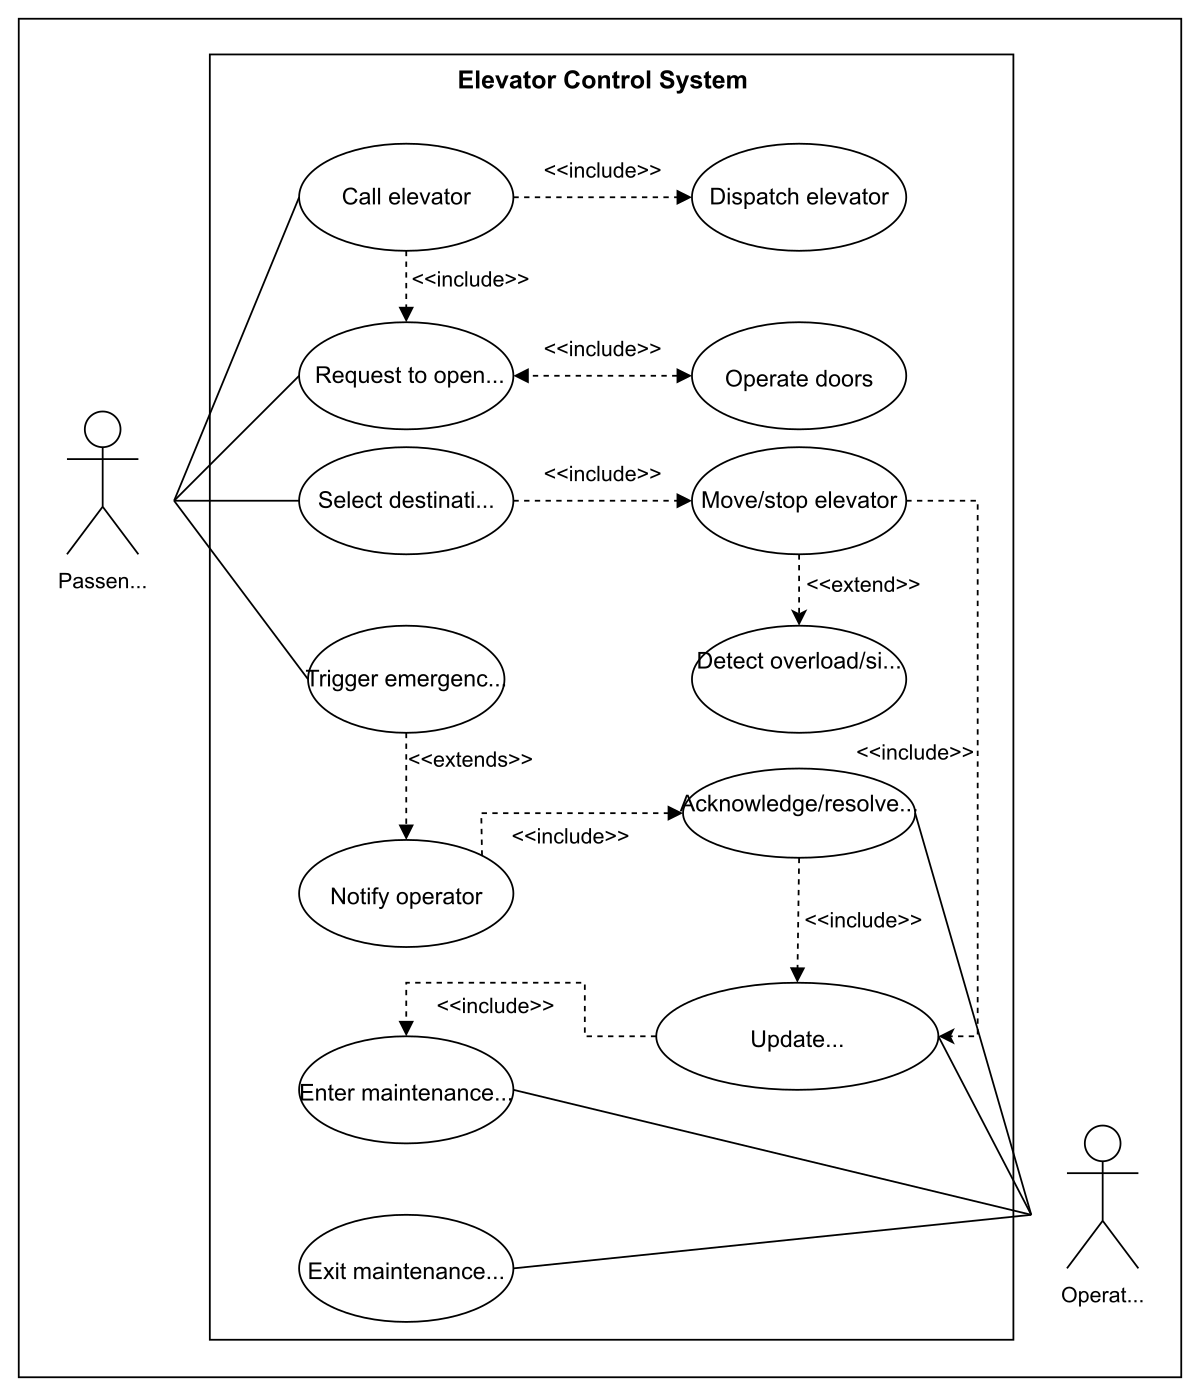
\includegraphics[width=0.5\textwidth]{Images/chapter_8/section_5060455555137536/4754801383309312.png}
 \caption{The use case diagram of the elevator system}
\end{figure}

In the next lesson, we will discuss the class diagram and explain all classes and their relationships.

% End of section content